\section{System Model}

\iffalse
\begin{figure}[t]
    \centering
      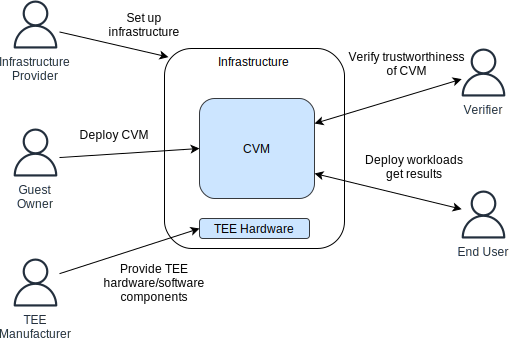
\includegraphics[width=.9\columnwidth]{figures/system-model.drawio.pdf}
    \caption{System Model and logical actors involved in the deployment of a
    \ac{CVM}.}
    \label{fig:system-model}
\end{figure}
\fi

In our system model, a guest owner deploys a \ac{CVM} on an infrastructure where
potentially other software is running at the same time, such as other VMs
(confidential or not), monitoring software, etc. The infrastructure is managed
by an infrastructure provider, and should provide the hardware and software
primitives required to run the \ac{CVM} in a \ac{TEE}. Besides, a verifier
performs attestation to make sure that the \ac{CVM} was deployed and booted
correctly; We refer to the IETF RATS architecture for a more comprehensive
representation of the attestation infrastructure~\cite{ietfRats}. Furthermore,
an end user interacts with the \ac{CVM} to, e.g., deploy workloads and retrieve
results. In general, some interaction between such actors is required and trust
relationships between them may vary according to the use case. Besides, two or
more logical actors can, in practice, be impersonated by the same party: For
example, when running a \ac{CVM} on a local machine, all actors may be played by
the owner of that machine. When deploying a \ac{CVM} in the cloud, however, all
actors are likely unique. We will discuss this scenario in more detail in
\cref{sec:scenario}.

In this paper, we follow the standard threat model of \acp{TEE}: All software
running outside of the \ac{CVM} is potentially malicious, including the
VMM/hypervisor, other VMs, etc. Note that this is true even when the guest owner
and the infrastructure provider are the same party or trust each other, since
the software running on the infrastructure might be compromised by remote
attackers. Instead, the \ac{TEE} manufacturer and any software and hardware
components provided by them are assumed to be secure. The \ac{TEE} threat model
mainly focuses on confidentiality and integrity but leaves out availability.
Additionally, side channels and physical attacks are also out of scope.

\subsection{The Importance of Remote Attestation}

\iffalse
\begin{figure}[t]
  \centering
    \includegraphics[width=.7\columnwidth]{figures/report.drawio.pdf}
  \caption{Representation of a generic \ac{TEE} attestation report. Information
  about the platform TCB and a digital signature bind the \ac{TEE} instance to a
  specific node. A \emph{launch measurement} along with a policy give
  information on the code and data running on the \ac{TEE} instance. User data
  may bind a credential owned by the \ac{TEE} instance to the attestation
  report. Finally, the report may contain other \ac{TEE}-specific fields that
  provide additional claims.}
  \label{fig:report}
\end{figure}
\fi

\begin{figure}[t]
  \centering
    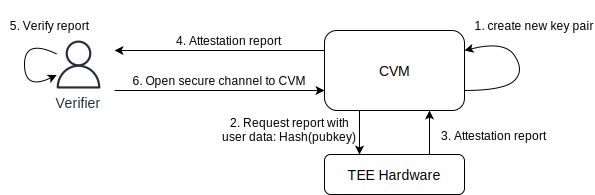
\includegraphics[width=.99\columnwidth]{figures/attestation-flow.drawio.pdf}
  \caption{High-level attestation flow.}
  \label{fig:attestation-flow}
\end{figure}

When it comes to \acp{TEE}, remote attestation is an essential step to gain
confidence in the deployed \ac{CVM}, making sure that, after boot:
\begin{inparaenum}
    \item the \ac{CVM} is running in a genuine and up-to-date \ac{TEE}, and
    \item the \ac{CVM} is in an expected and good state, i.e., only trustworthy
      and measured software has been loaded.
\end{inparaenum}
Moreover, attestation is often used to bind the identity of the \ac{CVM} to a
cryptographic credential, later used to establish a secure channel for
provisioning secrets and deploying workloads, e.g., via SSH or TLS connections.
Figure~\ref{fig:attestation-flow} shows how this is usually achieved.

After generating an ephemeral key pair (step 1), the \ac{CVM} embeds some
information about the credential in the attestation report requested from the
TEE hardware (step 2). This could include, e.g., a hash of the public ephemeral
key as well as a nonce provided by the verifier for freshness (not shown). The
signed attestation report returned by the TEE hardware (step 3) then includes
this data along with information about the TEE hardware and measurements of
software deployed in the TEE. After receiving and verifying the report (steps 4
\& 5), the verifier can now be certain that the key is \emph{owned} by a
\ac{CVM} with the specific hardware and software configuration matching the
attestation report.

When attestation fails, this binding becomes compromised, and the verifier (or
other entities) cannot be sure that they are communicating with a legitimate
\ac{CVM}. The problem is exacerbated by the complexity of \ac{CVM} attestation
that might lead to some components being accidentally skipped during
verification. In the next sections, we describe all steps of \ac{CVM}
attestation and show what might happen when some of these steps are missed.

\subsection{Attestation Levels}
\label{section:att-levels}

\begin{figure}[t]
    \centering
      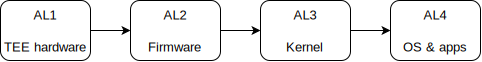
\includegraphics[width=.9\columnwidth]{figures/levels-v2.drawio.pdf}
    \caption{Hierarchy of attestation levels for \acp{CVM}.}
    \label{fig:attestation-levels}
\end{figure}

Attesting a \ac{CVM} is not an easy task since we need to ensure that every part
of the boot process is measured and can be verified. This section identifies
five stages of attestation of a \ac{CVM}, called \emph{Attestation Levels (ALs)}.
These levels are incremental, meaning that the guarantees provided at a certain
level build upon the levels below. A visual representation of such levels is
provided in \cref{fig:attestation-levels}.

\noindent\textbf{\emph{AL0: No attestation.}}
%
This is the baseline level where no attestation is done. As a result, the
verifier cannot make any claims on the state of the \ac{CVM} and the threat
model is the same as for a regular VM execution environment.

\noindent\textbf{\emph{AL1: Attested \ac{TEE} isolation.}}
%
In this level, the verifier has access to the ``raw'' attestation report signed
by the \ac{TEE} manufacturer, and is able to independently verify its integrity
and authenticity. This typically involves the verification of the report's
signature and certificate chain, which goes up to a root certificate that is
self-signed by the \ac{TEE} manufacturer. Moreover, the report also contains
some information about the platform's \ac{TCB} (e.g., CPU model, microcode
version, etc.), and freshness information provided by the verifier. This allows
the verifier to attest that the \ac{CVM} is indeed running in a genuine and
up-to-date \ac{TEE}, which reduces the threat surface significantly as the host
firmware, OS, and virtualization layer can now be excluded from the TCB. The
verifier can also be sure now that software running outside of the CVM cannot
directly access data stored inside of it. However, threats specific to the CVM
technology used, e.g., side channel leakage, or to the software running inside
the \ac{CVM} remain.   

\noindent\textbf{\emph{AL2: Measured firmware.}}
%
As mentioned above, remote attestation is used to establish a secure channel
into the \ac{CVM}, but AL1 does not give any information about what software is
running at the other end of that channel. A first step to alleviate this
situation is verify the \emph{launch measurement} contained in the attestation
report, which reflects the memory layout of the \ac{CVM} at boot time including
the firmware, page metadata and CPU register state. To obtain evidence for the
correct deployment of the firmware, the verifier needs to validate the launch
measurement against a trusted reference value. That measurement in itself does
not tell anything about the code and data running in the \ac{CVM}, hence it is
important that the firmware's source code is available and can be reproducibly
built.  After a successful verification, it can be ruled out that the trusted
firmware has been replaced by a malicious one.

\noindent\textbf{\emph{AL3: Measured Kernel.}}
%
To rule out compromise of later boot stages, the verifier needs to validate the
entire boot chain that starts from the firmware and goes up to the kernel,
(optionally) through a bootloader. This also includes the initial RAM disk and
kernel command-line parameters. By default, these components are not measured by
the \ac{TEE} and thus not part of the launch measurement. However, there are
several ways to make this attestation possible, some of which are discussed in
\cref{section:att-examples}.

\noindent\textbf{\emph{AL4: Fully measured boot.}}
%
The verification of the measurements done at AL3 stops at \emph{early
userspace}, i.e., right before the root filesystem is mounted to the \ac{CVM}.
At the very least, the root filesystem of the \ac{CVM} containing OS and
application data should be integrity protected, to prevent loading a malicious
version. In case it contains secrets, it should also be encrypted. The challenge
in this step is to securely provision keys to the \ac{CVM} only after a
successful AL3 attestation, to prevent leaking the keys to a compromised
\ac{CVM}. Again, possible implementation strategies are provided in
\cref{section:att-examples}.

After a successful AL4 attestation, the verifier has confidence that the desired
system and application software has been deployed correctly in the \ac{CVM}. At
this point, the threat model is similar to running the guest system on a trusted
dedicated server and run-time security of the \ac{CVM} is under the guest
owner's purview. In particular, the deployed software may employ security
policies to sanitize untrusted inputs or prevent the loading of additional,
untrusted software. Moreover, further attestation steps may be initiated by the
guest owner, e.g., run-time attestation of application control-flow integrity,
or attesting the authenticity of attached secure I/O devices.

\subsection{Attestation Strategies}
\label{section:att-examples}

Typically, support for AL1 and AL2 attestation is provided by all \ac{TEE}
manufacturers, via a certificate chain and a public key infrastructure (for AL1)
and a a measurement of the initial memory layout of the \ac{CVM} (for AL2). In
both cases, it is often sufficient to verify the attestation report that can be
fetched by the \ac{CVM} and sent to the verifier. To reach ALs 3 and 4, instead,
additional steps are needed. Below, we discuss possible approaches.

\noindent\textbf{\emph{AL3.}}
%
A simple strategy to make this attestation possible leverages Direct Linux Boot
to bind kernel measurements to the firmware, in such a way that the launch
measurement in the attestation report also reflects the identity of kernel
components~\cite{kernelHashesOvmf}. This can be done by adding kernel
measurements as firmware variables, which will be loaded into secure memory at
boot and measured by the \ac{TEE}. Then, the firmware will load and pass control
to the kernel only if its measurements match with the expected ones stored as
variables, aborting otherwise. A more involved solution involves relying on a
\ac{vTPM} for measuring the \ac{CVM} boot chain. On AMD SEV-SNP, this
functionality can be exposed thanks to \acp{VMPL}~\cite{AmdSevAbi}, where the
\ac{vTPM} executes in a higher privilege level than the rest of the system. To
bind \ac{vTPM} quotes to \ac{TEE} attestation reports, the digest of the
\ac{vTPM} endorsement key is added as user data in the \ac{TEE}
report~\cite{narayanan2023svsm}. The verifier, then, has to check both the
report and the quote to verify the trustworthiness of the \ac{CVM}. On Intel
\ac{TDX}, instead, a \ac{vTPM} can be exposed from a separate trust
domain~\cite{intelTdxvTPM}. Additionally, Intel \ac{TDX} also provides four
\acp{RTMR} whose value is reflected in the attestation
report~\cite{intelTdxModule}. These registers are analogous to a \ac{TPM}'s
PCRs, and can be similarly leveraged by a TDX-aware firmware to measure boot
components.

\noindent\textbf{\emph{AL4.}}
%
To ensure the integrity of the root filesystem, a common approach is to extend
the \ac{vTPM} measurements up to the user space with Linux
\ac{IMA}~\cite{sailer2004ima}. \ac{IMA} is a kernel subsystem responsible for
measuring all binaries that are loaded at runtime, and it supports remote
attestation. Measurements are stored in a measurement file which itself is
integrity-protected by a measurement stored in the TPM, to prevent tampering
from a privileged adversary. When adopting \ac{IMA}, it is important to be aware
that runtime measurements may be susceptible to time-of-check-time-of-use
attacks~\cite{bohling2020imatoctou}, and that there exist so-called
\emph{measurement gaps}, i.e., some components are not measured.

Another approach relies on protecting the integrity of the whole filesystem at
rest. 
%The Linux Kernel offers a functionality called \emph{device mapper}, for
%mapping physical block devices to higher-level virtual block devices. This
%mapping allows checking and/or modifying data in transit to and from the
%physical block devices, and can be leveraged to guarantee confidentiality,
%integrity and authenticity of a filesystem. 
To this extent, a popular software solution is \dmverity~\cite{dmVerity}, which
provides integrity protection by verifying the data blocks in a filesystem
against pre-computed hash values, stored as a Merkle tree on a separate disk.
The root of the tree (called root hash), guarantees integrity of the whole
filesystem, and must protected from tampering. In our attestation flow, the root
hash can be provided as a kernel parameter such that its integrity can be
verified with a AL3 attestation. Filesystems using \dmverity{} are mounted as
read-only; To enable both read and write, \dmintegrity{}~\cite{dmIntegrity} can
be leveraged instead to (re-)compute HMAC tags for each sector of the block
device. In this case, however, a key should be separately provisioned to the
kernel during early userspace. In our \ac{CVM} scenario, this means that
attestation should be performed during boot. Finally, \dmintegrity{} can be
combined with \dmcrypt{}~\cite{dmCrypt} to additionally provide encryption.

\subsection{Partial Attestation}
\label{section:partial-attestation}

\begin{figure}[t]
  \centering
    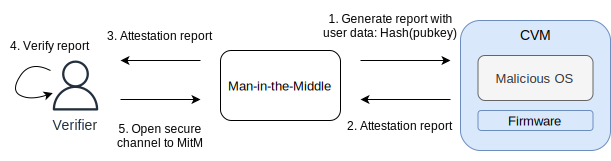
\includegraphics[width=\columnwidth]{figures/partial-attestation.drawio.pdf}
  \caption{Possible Man-in-the-Middle attack with an unverified guest OS.}
  \label{fig:partial-attestation}
\end{figure}


It should now be clear that attesting a \ac{CVM} is not a trivial task. Unlike
process-based \acp{TEE} such as Intel SGX, verifying the \ac{TEE} attestation
report alone is necessary but \emph{not sufficient} to cover the whole boot
process of the confidential workload. Failing to properly verify one or more
boot stages might cause some attacks to go undetected, such as injecting
malicious code or backdoors that would compromise the integrity and
confidentiality of the \ac{CVM}. These kind of attacks can be either local
(e.g., a compromised hypervisor tampering with the root filesystem) or remote
(e.g., a malicious kernel image downloaded from an untrusted
registry). Therefore, partial attestations might give a false sense of security
to guest owners and end users, who expect that their code and data is protected
when, in reality, this might not be true.

To showcase the severity of partial attestations, we consider the scenario where
the verifier only attests the \ac{CVM} up to AL2. Here, a \ac{MitM}
attack is possible if the \ac{CVM} loads a malicious OS
(\cref{fig:partial-attestation}): As the \ac{CVM} can produce attestation
reports with arbitrary user data, a \ac{MitM} that controls the \ac{CVM} OS can
bind the report with a credential owned by the \ac{MitM} (step 1). The verifier,
when receiving the attestation report (step 3), can successfully verify that the
report comes from a genuine \ac{CVM} with the expected firmware (step 4), but
cannot make any claims on the running OS. Failing to recognize this issue might
cause the verifier to bind the \ac{CVM} identity to the credential owned by the
\ac{MitM}, leading to the verifier possibly opening a channel with the \ac{MitM}
and leak secrets (step 5). What is worse, the \ac{MitM} does not even need to
run in a \ac{CVM}, meaning that all data will be processed in clear. Therefore,
although the verifier has performed a successful AL2 attestation, in
practice the security guarantees obtained are basically the same as without
attestation.
